\section{TCP/UDP}
TCP/IP階層モデルにおけるトランスポート層は,ネットワーク層で端末(ノード)間の橋渡しがなされ送られてきたパケットについて,これが届いたかどうかの確認をしたり,これの順序を整理したり,データが壊れていないかを確認したり,大きすぎるデータを分割したり,データの送信量を制御する.また,データを適切なアプリケーションに引き渡す役割もある.

トランスポート層の代表的なプロトコルとして,TCPとUDPがある.これら二つの違いをごく簡単に説明すると,信頼性のある通信を重視するものがTCP,伝送効率の高い通信を重視するものがUDPである,となる.

それではまず,UDPについて説明を始めよう.

\subsection{UDP}
UDPは,通信の信頼性よりも,速さやリアルタイム性が要求されるような場合において使用されるプロトコルである.UDPのヘッダを図\ref{tcpudp-udp-header}に示す.

\begin{figure}[htb]
  \centering
  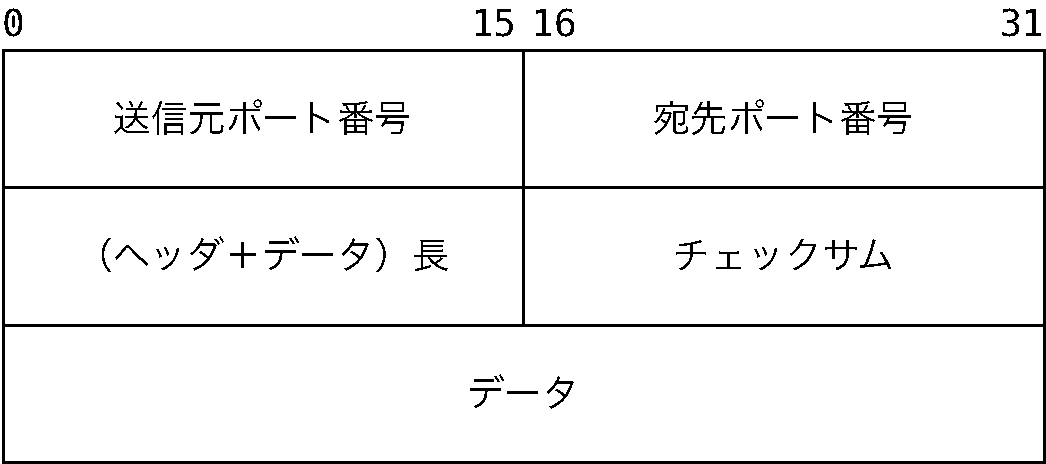
\includegraphics[bb=0 0 502 222, width=10cm]{tcpudp-udp-header.pdf}
  \caption{UDPヘッダ}
  \label{tcpudp-udp-header}
\end{figure}

UDPのヘッダは,このように極めてシンプルな構造になっている.データを転送する際,送信側はチェックサムの計算を行って送信するだけであり,受信側はチェックサムを計算してデータに誤りが無いか確認した後,受け取った順にそのままアプリケーションに渡すだけである.後述するTCPにおいて使われている3-way handshakeや確認応答,順序制御,再送制御,伝送制御などの機能は無く,処理がシンプルであるが故に高速なのである.

ただし,パケットが確実に到達するという保証が無いため,何らかの原因でパケットロスが発生した場合にでも処理を継続できるようにアプリケーション側で工夫する必要がある.

このプロトコルは,DNSやNTP,DHCPなどのデータ量の少ないものや,音楽や映画などのストリーミング配信,またオンラインゲームのようなリアルタイム性が要求されるもので使われることが多い.

\subsection{TCP}
TCPは,信頼性の高い通信を実現するために使用されるプロトコルである.TCPのヘッダを図\ref{tcpudp-tcp-header}に示す.シーケンス番号では送信するデータの通し番号を管理しており,確認応答番号(ACK番号)ではどのシーケンス番号までデータを受信したかを示している.

\begin{figure}[htb]
  \centering
  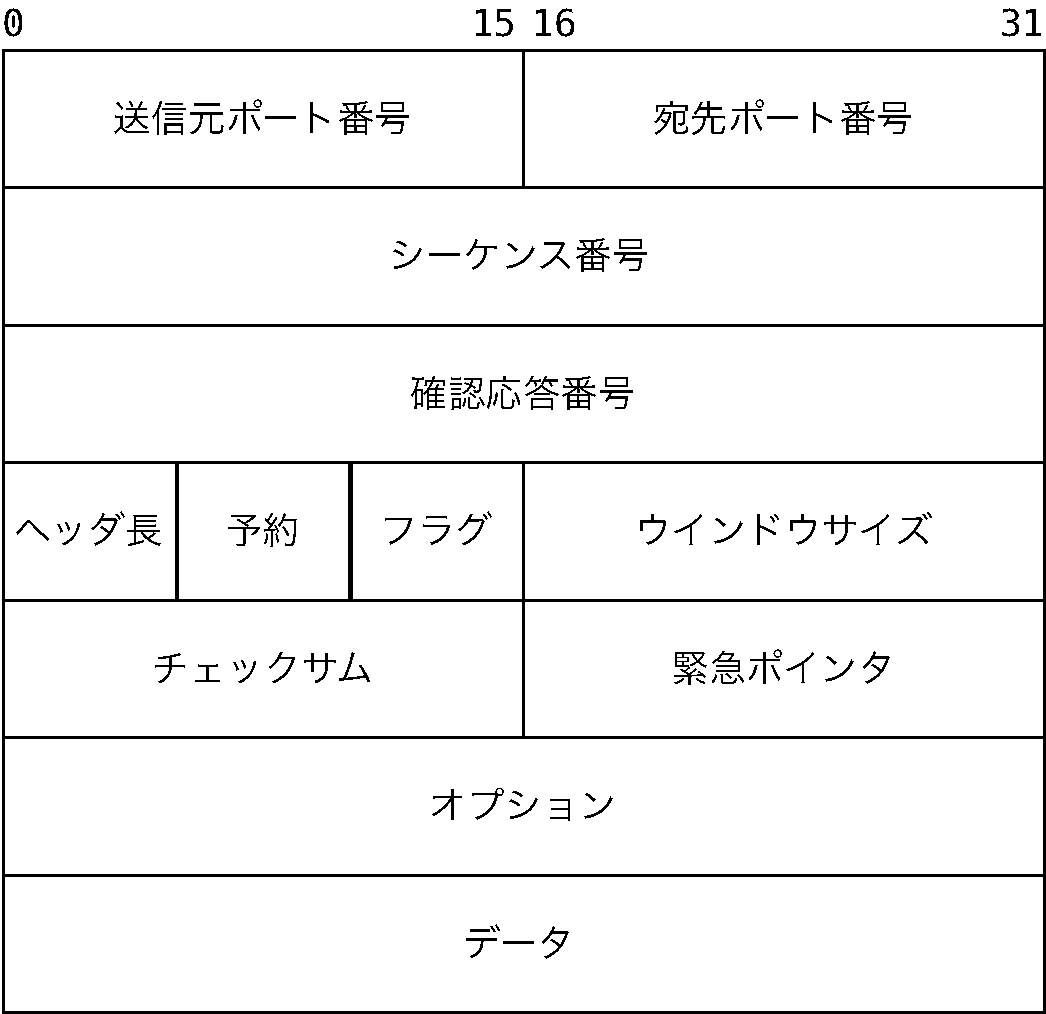
\includegraphics[bb=0 0 502 486, width=10cm]{tcpudp-tcp-header.pdf}
  \caption{TCPヘッダ}
  \label{tcpudp-tcp-header}
\end{figure}

フラグでは,そのTCPパケットがどのような種類のものなのかを示している.フラグ名とその意味を整理したものを表\ref{tcpudp-tcp-flaglist}に示す.

\begin{table}[htb]
  \centering
  \caption{TCPのフラグ一覧}
  \label{tcpudp-tcp-flaglist}
  \begin{tabular}{|c|l|} \hline
    URG & このTCPパケット内に緊急データが含まれていることを示す \\ \hline
    ACK & TCPヘッダ内に有効なACK番号が含まれていることを示す \\ \hline
    PSH & 受信したデータをすぐにアプリケーションに引き渡すよう要求する \\ \hline
    RST & TCP接続の中断,拒否を示す \\ \hline
    SYN & 3-way handshake時に使われ,ACK番号を同期させる \\ \hline
    FIN & TCP接続を終了させる \\ \hline
  \end{tabular}
\end{table}

また,TCPをベースとするHTTP通信の例を表\ref{tcpudp-http-sample}に示す.これを参考にしつつTCP通信の特徴を説明していく.

\begin{table}[htb]
  \centering
  \caption{HTTP通信の例}
  \label{tcpudp-http-sample}
  \begin{tabular}{|c|c|c|l|l|l|l|} \hline
      Src & Dst & Flag & Length & Seq num & Ack num & HTTP \\ \hline \hline
      Client & Server & SYN & 0 & 0 & 0 & \\ \hline
      Server & Client & SYN,ACK & 0 & 0 & 1 & \\ \hline
      Client & Server & ACK & 0 & 1 & 1 & \\ \hline
      Client & Server & PSH,ACK & 394 & 1 & 1 & \shortstack{GET /$\sim$bob/sample.html \\ HTTP/1.1} \\ \hline
      Server & Client & PSH, ACK & 353 & 1 & 395 & HTTP/1.1 200 OK \\ \hline
      Client & Server & ACK & 0 & 395 & 354 & \\ \hline
      Server & Client & FIN,ACK & 0 & 354 & 395 & \\ \hline
      Client & Server & ACK & 0 & 395 & 355 & \\ \hline
  \end{tabular}
\end{table}

まず,TCPではUDPのようにデータを一方的に送りつけるのではなく,事前に接続を確立する手順を踏む.この手順のことを3-way handshakeと呼ぶ.表\ref{tcpudp-http-sample}の例では上から三つ分のパケットがこれにあたる.

まず,接続する側(クライアント)は接続される側(サーバ)に対してSYNフラグを立てたパケットを送信し,上りのコネクション確立を試みる.これを受け取ったサーバ側はACKとSYNフラグを立てたパケットを送信し,上りのコネクション確立を承認するとともに,下りのコネクション確立を試みる.これを受け取ったクライアント側はACKフラグを立てたパケットをサーバに送信し,下りのコネクション確立を承認する.以上の手順により信頼性のあるコネクション確立が完了し,これ以降でデータの通信が行われる.

送信したデータが全て受信側に到着したかを確認するために,データのバイト数とシーケンス番号,ACK番号が用いられる.例として送信側が394バイトのデータを送信するケースを考えてみる.送信側はデータと共にシーケンス番号を送信する.これを受け取った側はデータのバイト数とシーケンス番号を足し,これをACK番号として送信側に送る.これを受け取った送信側で,受け取ったACK番号が,送信したデータのバイト数と送信時のシーケンス番号を足したものと一致していれば全てのデータが到達していることがわかる.もしここで数値が一致しなければ,再度データを送信することになる.

\subsubsection{パケット転送効率の改善}
上述の通り,TCPではパケットを送信し,ACKを受け取るという流れを繰り返してデータ転送を行う.だがこのままだとパケット送信からACK受信までの時間(RTT,Round Trip Time)の関係で,送信側で送信準備ができていたとしてもACKを受け取れない限り送信できず,転送の効率が悪化する.

これを改善するために,TCPではウインドウ制御の一つの方法である,スライディングウインドウ方式という仕組みがある.TCPヘッダの中にはウインドウサイズという,受信側が受信できるデータ量を送信側に知らせるフィールドがある.送信側はこのウインドウサイズをもとに,ACKを待たずに次々にパケットを送信する.一定量パケットを送信したらACKパケットを待ち,ACKパケットを受け取ったらまた次のパケットを送っていくという方法になる.ウインドウサイズに収まるサイズのデータを送り,どこか一つのパケットに対応するACKを受信したらそこまでのパケットは到達しているとみなしてウインドウを横にずらして新たなパケットを送信するイメージである.

スライディングウインドウ方式により,送信側の転送効率は上がる.だがこれではネットワークの混雑度合いを考慮できておらず,次々にパケットを送信し続けてしまうことで混雑度合いをさらに悪化させてしまう.この問題に対処するために,輻輳制御という方法が用いられている.初めからウインドウサイズ一杯でパケットを送信するのではなく,徐々に転送量を増やしていき,輻輳が発生した場合に再度ウインドウサイズを小さくして再度転送量を増やすというものだ.

以上の仕組みはパケットの送信側において,効率よくパケットを送信するための仕組みである.ただ,パケットの受信側で処理に時間がかかるような場合,次々にパケットを送信されてしまうと受信側は処理がパンクしてしまう恐れがある.これを回避するためにもウインドウサイズは用いられる.パケットが送られてくるたびにウインドウサイズを減らして送信側に通知し,処理がパンクしそうになるとウインドウサイズをゼロにして送信側に通知する.これにより送信側は受信側の状況を見てパケットの送信を中断でき,受信側で余裕ができたらこれを通知して通信を再開させたり(ウインドウ更新通知),送信側が受信側に余裕ができたかを問い合わせて通信を再開することができる(ウインドウプローブ).

以上のような仕組みを用いてTCPは転送効率の向上を行っている.

\subsection{チェックサム}
TCPやUDP(とIP)にはチェックサムという仕組みがあり,これを用いてデータの損傷を検出できるようになっている.計算に用いるのは,TCPあるいはUDPヘッダとデータ,擬似ヘッダの三つである.擬似ヘッダとは仮想的なヘッダで,実際のTCPパケット内には含まれておらず,チェックサムを計算する際にのみ利用する.

送信側は,まずTCPあるいはUDPヘッダとデータ,擬似ヘッダの三つで合わせて16ビットの整数倍になるようにデータの長さを調節する.また,あらかじめチェックサムフィールドをゼロで埋めておく.そして先ほど調節したデータとTCPあるいはUDPヘッダ,擬似ヘッダについて16ビットごとに1の補数を求め(ビット反転させ),その総和を求め,これの1の補数をチェックサムフィールドに入れて送信する.
受信側は,同様に擬似ヘッダを付けた状態で16ビットずつ1の補数を求め,その総和を計算する.データが破損していない場合はこの計算結果が0xFFFFになる.これは送信側がチェックサムフィールドに入れた値がチェックサムフィールド以外の補数和の1の補数であり,受信側が行っていることはチェックサムフィールド以外の補数和にその1の補数を足す処理をしている,ということから分かるのではないかと思う.

\subsection{ポート番号}
TCP/IP階層モデルにおけるトランスポート層ではアプリケーション層との間でのデータのやり取りを担うが,どのアプリケーションからのデータなのか,また,どのアプリケーションに対してのデータなのかを識別するためにポート番号が用いられる.ポート番号はTCPとUDPでそれぞれ0番から65535番まであり,その中で大きく三つの種類に分けられる.この分け方を表\ref{tcpudp-kind-of-port}に示す.
\begin{table}[htb]
    \centering
    \caption{ポート番号の種類}
    \label{tcpudp-kind-of-port}
    \begin{tabular}{|c|c|} \hline
        Well Known Ports & 0 $\sim$ 1023 \\ \hline
        Registered Ports & 1024 $\sim$ 49151 \\ \hline
        Dynamic and/or Private Ports & 49152 $\sim$ 65535 \\ \hline
    \end{tabular}
\end{table}

まず,0番から1023番まではWell Known Ports(System Ports)と呼ばれ,例えばSSH(22)やHTTP(80),HTTPS(443)などの一般的によく利用される主要なサービスのために登録されている.また,Unix系OSにおいてこの範囲のポートは管理者の権限を持つユーザのみが利用できる.1024番から49151番まではRegistered Ports(User Ports)と呼ばれ,一般的なサービスではないが,登録制によって割り当てられるものとなる.49152番から65535番まではDynamic and/or Private Portsと呼ばれ,クライアント側で自動的に利用されるもの,あるいはユーザが自由に利用できるもの,とされている.
これらポート番号の管理や割り当ては,IANA(Internet Assigned Numbers Authority)が行っている.

